% Preamble
% Compile with XeLateX

\documentclass[5pt,oneside,a4paper,titlepage]{article}
\usepackage{preamble}
\graphicspath{{PIC/}}
%%%%%%%%%%%%%%%%%%%%%%%%%%%%%%%%%%%%%%%%%%%%%%%%%%%%%%%%%%%%%%%%%%%%%%%%%%%%%%%%%%%%%%
\begin{document}

\sidebar{sideBarColor!25}
\simpleheader{titleBackColor}{Tich}{Zvidzayi}{Full Stack - Software Engineer}{white}

% Start Minipages
\vspace*{3.49cm}% start 8 cm from the top of the page}
    \adjustbox{valign=t}{\begin{minipage}{7.3cm} % large 7.4 cm from the top
    \vspace*{1.2cm} % text starts 1cm under the top of the minipage
            
        % Picture
        \begin{center}
        \begin{tikzpicture}
            \node[
            circle,
            minimum size=\cvPictureWidth,
            path picture={
            \node at (path picture bounding box.center){
             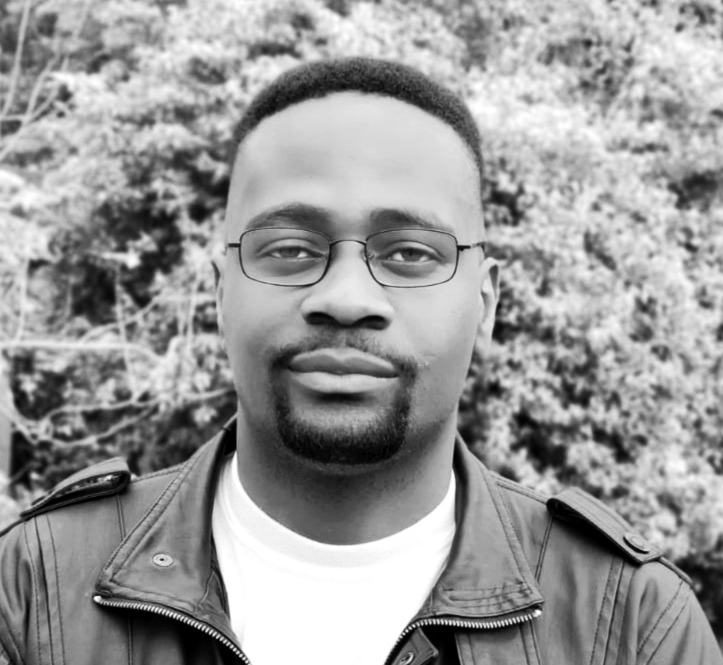
\includegraphics[width=\cvPictureWidth]{Picture.jpeg}
             };
             }]
            {};
        \end{tikzpicture}
        \end{center}

        %%%%%%%%%%%%%%%%%%%%%%%%%%%%%%%%%%%%%%%%%%%%%%%%%%%%
        % Profile section
        \vspace*{1.5cm}
        \ruleline{\textbf{About Me}}
        Tich is a Software Engineer (Full Stack ) with over two years of experience. Tich has worked with technologies like Java, ASP.NET (C\#), PHP, Laravel, and JavaScript (VueJS, ReactJS, JQuery, NodeJS). He is also keen on picking up other technologies like Angular, Django, Golang and Scala. Tich holds a BSc, BSc Honours and Masters in Computer Science degrees from Rhodes University. Tich is also a member of the Golden Key Society. Tich won a sparring gold medal in Taekwondo ITF national competition in 2014. Tich prefers an organisation with a culture growth, creativity and transparency.
        
        %%%%%%%%%%%%%%%%%%%%%%%%%%%%%%%%%%%%%%%%%%%%%%%%%%%
        % Contact Section
         \vspace*{1.5cm}
        \ruleline{\textbf{Personal Information}} \\
        \begin{tikzpicture}[every node/.style={inner sep=0pt, outer sep=0pt}]
        \matrix [
        column 1/.style={anchor=center,contactIcon},
        column 2/.style={anchor=west,align=left,contactIcon},
        column sep=5pt,
        row sep=5pt] (contact) {
      
        \node{\faEnvelope}; 
         & \node{{tzvidzayi@hotmail.com}};\\
         \node{\faEnvelopeO}; 
    
        \node{\faPhone}; 
         & \node{+27 63 323 8051};\\ 
        \node{\faMapMarker}; 
        & \node{Cape Town (Parklands) \\South Africa};\\ \\
        \node{\faGithub}; 
        & \node{https://github.com/tichzvidzayi};\\ 
       \\  };
        \end{tikzpicture} 
        
        %%%%%%%%%%%%%%%%%%%%%%%%%%%%%%%%%%%%%%%%%%%%%%%%%%%
         \vspace*{1.5cm}
        \ruleline{\textbf{Languages}}
        \begin{tikzpicture}[every node/.style={inner sep=0pt, outer sep=0pt}]
        \matrix [
        column 1/.style={anchor=center,contactIcon},
        column 2/.style={anchor=west,align=left,contactIcon},
        column sep=5pt,
        row sep=5pt] (contact) {
        \node{\flag{England.png}};
        & \node{English - Professional Knowledge};\\
        & \\
        }; \end{tikzpicture} 
        
 %%%%%%%%%%%%%%%%%%%%%%%%%%%%%%%%%%%%%%%%%%%%%%%%%%%%%
        % QR Code
      
        
    \end{minipage}} %
    \hfill 
%%%%%%%%%%%%%%%%%%%%%%%%%%%%%%%%%%%%%%%%%%%%%%%%%%%%%%%%%
%%%%% MAIN SECTION %%%%%%%%%%%%%%%%%%%%
    \adjustbox{valign=t}{\begin{minipage}{11.3cm}
        \vspace*{1cm}

         % Work Experience
        \section*{{\faSuitcase} WORK EXPERIENCE}
        %%%%%KITS
        \MySectionNoPic{October 2022- present}{Software Engineer}{ }{KITS}{KITS is a German-based legal automation company.\\ Responsibilities:
        \begin{itemize}
            \item Worked as part of a small team to automate legal services for clients in Europe.
            \item Participated in code peer reviews to ensure clean and efficient code. 
            \item Used an Agile two-week Sprint and daily stand-ups (daily progress report)  
        \end{itemize}
        
        \textbf{Technologies} C\#/ASP.Net |BPMN | JavaScript|React|NodeJS| ExpressJS|jQuery|Jira Software|Git
        }
       \\ 
       \\
       
        %%%%%%%%Pargo%%%%%%    
        \MySectionNoPic{January 2022- November 2022}{Software Engineer}{Cape Town, South Africa}{Pargo Pty}{Pargo is a smart-logistics company that simplifies last-mile logistics.\\ Responsibilities:
        \begin{itemize}
            \item Worked with other software engineers, testers, and product owners to identify problems, formulate and code solutions. 
            \item Participated in code peer reviews to ensure clean and efficient code. 
            \item Used an Agile two-week Sprint and daily stand-ups (daily progress report)this also included casual Tech talks to stay up-to-date with emerging technologies. 
            \item Engineered new features that helped Pargo to expand its products and provide better services to customers.
        \end{itemize}
        
        \textbf{Technologies} PHP|Laravel | JavaScript| VueJS|NodeJS| Docker | Jira Software | Grafana Monitoring| Sentry| PostgresSQL | InfluxDB | Git (Github)
        }

    %%%%%%%%%%%%%%%%Insight Technologies %%%%%%%%%%%%%%%%%%     
        \vspace*{0.5cm}
       \MySectionNoPic{November 2019 - August 2020 }{Back-end Developer}{Grahamstown, South Africa}{Insight Technologies }{ Insight Technologies is an IT consulting company and I worked for their client (nisc.co.za) an African journal publishing company. \\ Responsibilities:
        \begin{itemize}
           \item Worked closely with the director to identify requirements, formulate solutions and set milestones with clear deliverable.
          \item Maintaining, developing new features, and troubleshooting errors that occur in production.
           \item Used a weekly review to address progress, challenges, and improvements.
        \end{itemize}
        
        \textbf{Technologies} Java| MySQL | JavaScript | JQuery | PHP | Git.
        
        }
   \vspace*{0.2cm}

%%%%%%%%%%%%%%%%%%%%%%%%%%%%%%%%%%%%%%%%%%%%%%%%%%%%%%%%%%%%%%

       \vspace*{0.5cm}
       \MySectionNoPic{August 2020 - November 2021 }{Assistant Lecturer}{Grahamstown, South Africa}{Rhodes University }{ Rhodes University is a South African and internationally recognised university \\ Responsibilities:
        \begin{itemize}
           \item Worked closely with the lecturer and department secretaries to facilitate Computer Science modules.
           \item Responsible for setting practicals and invigilating exams
       
        \end{itemize}
          \textbf{Technologies} C\# | JavaScript | Spreadsheets | UX Design | SQL.
        
        
        }
   \vspace*{0.2cm}

%%%%%%%%%%%%%%%%%%%%%PeopleSmart%%%%%%%%%%%%
         \vspace*{0.5cm}
       \MySectionNoPic{January 2018 - November 2018 }{Software Developer}{Harare, Zimbabwe}{PeopleSmart Human Capital Consultant (prev. Masani)}{ PeopleSmart Human Capital Consultants is a consultancy organisation specialising in connecting businesses to employers. \\ 
       Responsibilities:
        \begin{itemize}

            \item Worked as part of a young team to develop C\# WPF desktop applications to simplify business solutions.
            \item Helped with testing of specific software products.     
        \end{itemize}
        \textbf{Technologies} Java | C\# / ASP.NET | JavaScript| Git
        }
        
   \vspace*{0.20cm}
%%%%%%%%%%TA Rhodes UNI%%%%%%%%%%%%%%%%%%%%%%%
\end{minipage}} %
%%%%%%%%%%
% Second Page
\newpage
\sidebar{sideBarColor!25}https://www.overleaf.com/project/637da2d1f073a7f688dfdf33
\newpageheader{titleBackColor}{Tich}{Zvidzayi}{Software \faLightbulbO \hspace{1mm} Engineer}{white}

% %%%%%%%%%%%%%%%%%%%%%%%%%%%%%%%%%% SIDEBAR %%%%%%%%%%%%%%%%%%%
\adjustbox{valign=t}{%
\begin{minipage}{7.3cm} 
\vspace*{0.4cm} % text starts 0.4cm under the top the header
        
%%%%%%%%%%%%%%%%%%%Skill and Strengths%%%%%%% 
 \vspace*{0.50cm} 
    \ruleline{\textbf{Soft Skills and Strengths}}
    \vspace*{-0.5cm}
    \begin{center}
       \cvtag{Adaptability} \cvtag{Attention to Details}\cvtag{Keen to Learn }\cvtag{Team Work}
    \end{center}
%%%%%%%%%%%%%%%%%%%%%%%%%%%%%%%%%%%%%%%%%%%%%%%%%%%
    % Professional Skills 
     \vspace*{0.9cm}
    \ruleline{\textbf{Technical Proficiency}}
    \begin{center}
        \cvtag{JavaScript} \cvtag{ReactJS} \cvtag{VueJS} \cvtag{NodeJS} \cvtag{JQuery}\cvtag{PHP} \cvtag{Laravel}\cvtag{C\#}\cvtag{Java} \cvtag{F\#}\cvtag{ SQL} \cvtag{Python} \cvtag{ASP.Net} \cvtag{Git} \cvtag{Shell Scripting}
    \end{center}

    %%%%%%%%%%%%%%%%%%%%%%%%%%%%%%%%%%%%%%%%%%%%%%%%%%%
    % Other Interests
     \vspace*{0.9cm}
    \ruleline{\textbf{Other Interests}}
    \small
    \begin{multicols}{2}
        \begin{itemize} 

            \item  SDN
            \item  Blockchain
            \item  ICT4D
            \item Taekwondo
            \item  Animation 
            \item Astronomy
       
    \end{itemize}
    \end{multicols}

     %%%%%%%%%%%%%%%%%%%%%%%%%%%%%%%%%%%%%%%%%%%%%%%%%%%%%
        % QR Code

\end{minipage}
}%
\hfill
%%%%%%%%%%%%%%%%%%%%%%%%%%%%%%%%%%% MAIN %%%%%%%%%%%%%%%%%%%%%%%%%
\adjustbox{valign=t}{%
\begin{minipage}{11.3cm} 

%%%%%%%%%%%%%%%%%%%%%%%%%%%%%%Projects
\vspace*{0.40cm}
\section*{{ \faGithub}  Personal Projects}
    \begin{itemize}
        \footnotesize
         \item{ \textbf{tOrdersAPI}\\{An API for storing and retrieving items that are stored. The API was tested using the Postman application.\\ \textbf{Technologies}: Python, Flask, REST API, HTML, CSS (Bootstrap).  \\ \textit{Available on}: https://github.com/tichzvidzayi/tOrdersAPI };
 }

     \item{\textbf{UserManagementSystem}\\{A web-application based user management system. This project can be extended to a full-blown school management system that can store academic, and credit records, etc.\\ \textbf{Technologies}: PHP and Laravel, HTML, CSS (Bootstrap), JavaScript (VueJS) \\  \textit{Available on}: https://github.com/tichzvidzayi/UserManagementSystem }
 }
\item {\textbf{FlipCardMemoryGame} \\ A Reactjs FlipCardMemory Game\\
\textbf{Available on}: https://github.com/tichzvidzayi/FlipCardMemoryGame}

 \item{\textbf{tMediaPlayer}\\{A desktop application for playing media content e.g., mp3, mov, mp4, avi.\\ \textbf{Technologies}: C\# and Windows Forms.  \\ \textit{Available on}: https://github.com/tichzvidzayi/tMedia-Player};
 }
\item {\textbf{BookStore API} \\ A C\# ASP.Net BookStore API\\
\textbf{Available on}: https://github.com/tichzvidzayi/BookStoreAPI}

 \item{\textbf{tURLshortener}\\{ A web application that shortens long URLs to short URLs. 
\\ \textbf{Technologies}: PHP, JavaScript, JQuery, MySQL, Apache server, CSS.  \\ \textit{Available on}: https://github.com/tichzvidzayi/tURLshortener};
 }


 \end{itemize}

%%%%%%%%%%%%%%%%%%%%%%%%%%ACADEMIC%%%%%%%


    \section*{{\faGraduationCap} EDUCATION}

        \MySection{ \faGraduationCap}{rhodes.png}{Master Degree in Computer Science}{Rhodes University}{South Africa}{Research: on the Linux Terminal Server Project (LTSP)to support ICT4D. \\\textit{Year: Feb 2019 - July 2021}}
   
        \vspace*{0.22cm}
            
        \MySection{\faGraduationCap}{rhodes.png}{BSc in Information Systems with Honours}{Rhodes University}{South Africa}{ Research: Artificial Intelligence. \\\textit{Year: 2013 - 2017}}
                
           
        \MySection{\faGraduationCap}{rhodes.png}{BSc in Information Systems }{Rhodes University}{South Africa}{\\\textit{Year: 2013 - 2017}}




%%%%%%%%%%%%%%%%%%%%%%%%%%%%%%%%%%%
    \vspace*{0.4cm}
    %%%%%%%%%%%%%%%%%%%%%%%%%%%%%%%%%%%%%%%%%%%%%%%%%%%
    % Peer Reviews
    \section*{{\faBook} ACADEMIC PUBLICATIONS}
    \begin{itemize}
        \footnotesize
         \item{IST Africa 2021 Conference: LTSP client image maintenance: Utilising a virtualisation player to support educators to directly manage classroom applications (presented), March 2021;}
     \end{itemize}
        
    %%%%%%%%%%%%%%%%%%%%%%%%%%%%%%%%%%%%%%%%%%%%%%%%%%%
    % Certificates
    \section*{{\faCertificate} CERTIFICATES}

    \begin{itemize}
        \item Udemy: Microsoft Azure DevOps \& Amazon Web Service DevOps Masterclass 2 Course Bundle.
        \item LinkedIn:Building Web API with ASP.NET Core in .NET 6
        \item LinkedIn: ReactJs Essential Training
        \item Complete Linux Training Course
        \item Coursera: (University of Minnesota) Introduction to
Software Testing.
        \item Coursera: (University of Alberta) Software Processes
and Agile Practices. 
    \end{itemize}
 
\end{minipage}}


%%%%%%%%%%
% Third Page
 %% \newpage
%%kkkk
\end{document}
